\section{Matrix-based multiple-source CFPQ algorithm}
\label{sec:multiple-source-algo}

 In this section we introduce two versions of multiple-source matrix-based CFPQ algorithm.
 This algorithm is a modification of Azimov's matrix-based algorithm for CFPQ and its idea is that we cut off those vertices from which we are not interested in paths.
 

In order to simplify Azimov's algorithm modification and the final algorithm description, we simplify the input graph to have only edge labels.
Note, that we always can convert the original graph into such form. 
To do it we should add loops into vertices in the following way: for the vertex $i$ we add an edge $i \xrightarrow{x} i$ iff $\lambda_V(i) = x$ and $x\neq \varnothing$.
This way we can switch to edge-labeled graph with the same number of vertices with preserving of the defined semantics of CFPQ.

\begin{figure}[h]
    \centering        
    \begin{tikzpicture}[shorten >=1pt,auto]
       \node[state] (q_0)                        {$0$};
       \node[state] (q_1) [right=of q_0]         {$1$};
       \node[state] (q_2) [below left=of q_1]    {$2$};
       \node[state] (q_3) [below left=of q_2]    {$3$};
       \node[state] (q_4) [below right=of q_2]   {$4$};
       \node[state] (q_5) [below right=of q_1]   {$5$};
       \path[->]
        (q_0) edge[loop left]  node {$\{x, y\}$} (q_0)
        (q_0) edge  node {$\{a\}$} (q_1)
        (q_2) edge[loop left]  node {$\{x\}$} (q_2)
        (q_1) edge  node {$\{b\}$} (q_5)
        (q_1) edge  node {$\{a, b\}$} (q_2)
        (q_3) edge[above]  node {$\{c\}$} (q_2)
        (q_4) edge  node {$\{c\}$} (q_3)
        (q_2) edge[above]  node {$\{c\}$} (q_4)
        (q_4) edge[loop below]  node {$\{y\}$} (q_4)
        (q_5) edge[bend left, below]  node {$\{d\}$} (q_4)
        (q_4) edge[bend left, above]  node {$\{d\}$} (q_5);
    \end{tikzpicture}
    \caption{The example of $D_1'$: the modified input graph $D_1$}
    \label{fig:example_modified_input_graph}
\end{figure}

The adjacency matrix $M$ of the graph $D_1'$ is
$$
    M =
    \begin{pmatrix}
    \{x, y\}     & \{a\} &   \varnothing      &   \varnothing   &   \varnothing   &   \varnothing   \\
    \varnothing     &   \varnothing   & \{a, b\} &   \varnothing   &       & \{b\} \\
    \varnothing     &   \varnothing   &   \{x\}      &   \varnothing   & \{d\} &   \varnothing   \\
    \varnothing     &   \varnothing   & \{c\}    &   \varnothing   &   \varnothing   &   \varnothing   \\
    \varnothing     &   \varnothing   &   \varnothing      & \{c\} &   \{y\}   & \{d\} \\
    \varnothing     & \varnothing     &   \varnothing      &   \varnothing   & \{d\} &   \varnothing
    \end{pmatrix}.
$$

Note that this transformation is impractical for real-world graphs, thus we use it only for algorithm description.

The first version of multiple-source algorithm is the Azimov's algorithm equipped with vertices filtering.
Let $G = (N, \Sigma, P, S)$ be the input context-free grammar, $D = (V, E, \Sigma_V, \Sigma_E, \lambda_V, \lambda_E)$ be the input graph and $Src$ be the input set of start vertices.
The result of the algorithm is a Boolean matrix which represents relation $R_{S,D}^{Src}$.

\begin{algorithm}
\begin{algorithmic}[1]
\caption{Multiple-source context-free path querying algorithm}
\label{alg:algo1}
\Function{MultiSrcCFPQ}{$D = (V, E, \Sigma_V, \Sigma_E, \lambda_V, \lambda_E),~G=(N,\Sigma,P,S), Src$}
    \State{$T \gets \{T^A \mid  A \in N, T^A \gets \varnothing\}$}
    \Comment{Matrix in which every element is $\varnothing$}
    
    \State{$TSrc \gets \{TSrc^A \mid  A \in N, TSrc^A \gets \varnothing\}$}
    \Comment{Matrix for input vertices in which every element is $\varnothing$}

    \ForAll{$ v \in Src$} \Comment{Input matrix initialization}
        \State{$TSrc^S_{v,v} \gets true$} 
    \EndFor

    \ForAll{$A \to x \in P$} \Comment{Simple rules initialization}
        \ForAll{$(v, to) \in E, \lambda_E(v,to) = x$}
            \State{$T^A_{v,to} \gets true$}
        \EndFor
    \EndFor

    \While{$T\ or\ TSrc\ is\ changing$} \Comment{Algorithm's body}
        \ForAll{$A \to B C \in P$}
            \State{$M \gets TSrc^A*T^B$}
            \State{$T^A \gets T^A + M*T^C$}
            \State{$TSrc^B \gets TSrc^B + TSrc^A$}
            \State{$TSrc^C \gets TSrc^C + $ \Call{getDst}{$M$}}
        \EndFor
    \EndWhile
    \State \Return $T^S$
\EndFunction

\\

\Function{getDst}{$M$}
    \State{$A \gets \varnothing$}
    \ForAll{$(v,to) \in V^2 \mid M_{v,to} = true$}
        \State{$A_{to,to} \gets true$}
    \EndFor
    \State \Return A
\EndFunction
\end{algorithmic}
\end{algorithm}

In order to solve the single-source and multiple-source CFPQ problem Azimov's algorithm was modified: each time, when we apply grammar rule (Boolean matrix multiplication $T_A = T_A + T_B \cdot T_C$ for each $A \rightarrow BC \in P$ represented in line \textbf{8} of Algorithm~\ref{alg:algo0}) we should save only vertices of interest. 
To do it, matrix multiplication was supplemented with one more matrix multiplication $T_A = T_A + (TSrc^A \cdot T_B) \cdot T_C$, where $TSrc^A$ --- matrix of vertices to calculate the paths from (lines \textbf{11-13} of the Algorithm~\ref{alg:algo1}).
Also, after every iteration of while loop this is necessary to update the set of vertices paths from which we need to calculate. 
To do this, the function \textbf{getDst}, represented in lines \textbf{17-21}, is called at line \textbf{14}.
Thus, the modified algorithm supports the frontier of the actual vertices and updates it on each iteration.
As a result it does not calculate the paths from all vertices in case of query to calculate the paths small set of vertices.

========================
We proposed the variant of the algorithm that can calculate the paths from a certain set of vertices, however there are such scenarios when queries are partially or completely repeated. In such cases it would be useful to add data caching to improve the performance. The problem is that every time we want to find all paths from the certain set of vertices, the Algorithm~\ref{alg:algo1} calculates everything from scratch. Since recalculating might take the significant amount of time, we modified multiple-source CFPQ algorithm to specify it for such scenarios. This version stores all the vertices the paths from which have already been calculated in cash $index$, which is used to filter such vertices in line \textbf{3} of Algorithm~\ref{alg:algo2}. Thus, modified algorithm calculates paths from the particular vertex only once.
\begin{algorithm}
\begin{algorithmic}[1]
\caption{Optimized multiple-source context-free path querying algorithm}
\label{alg:algo2}
\Function{CreateIndex}{$D = (V, E, \Sigma_V, \Sigma_E, \lambda_V, \lambda_E),~G=(N,\Sigma,P,S)$}
    \State{$T \gets \{T^A \mid  A \in N, T^A \gets \varnothing\}$}
    
    \State{$TSrc \gets \{TSrc^A \mid  A \in N, TSrc^A \gets \varnothing\}$}
    
    \ForAll{$A \to x \in P$} \Comment{Simple rules initialization}
        \ForAll{$(v, to) \in E, \lambda_E(v,to) = x$}
            \State{$T^A_{v,to} \gets true$}
        \EndFor
    \EndFor
    
    \State $index = (\mathcal{D}, \mathcal{G}, T, TSrc)$
    \State \Return $index$
\EndFunction

\Function{MultiSrcCFPQSmart}{$index, Src$}
    
    \State{$TNewSrc \gets \{TNewSrc^A \mid  A \in N, TNewSrc^A \gets \emptyset\}$}

    \State{$S = index.\mathcal{G}.S$}
    \ForAll{$v \in Src \mid index.TSrc_{v,v} = false$}
        \State{$TNewSrc^S_{v,v} \gets true$}
    \EndFor

    \While{$index.T\ or\ TNewSrc\ is\ changing$}
        \ForAll{$A \to B C \in P$}
            \State{$M \gets TNewSrc^A*index.T^B$}
            \State{$index.T^A \gets index.T^A + M*index.T^C$}

            \State{$TNewSrc^B \gets TNewSrc^B + TNewSrc^A \setminus index.TSrc^B$}
            \State{$TNewSrc^C \gets TNewSrc^C + $ \Call{getDst}{M}} $\setminus$ $index.TSrc^C$
        \EndFor
    \EndWhile
\EndFunction


\end{algorithmic}
\end{algorithm}

\subsection{Implementation Details}

 All of the above versions have been implemented$\footnote{GitHub repository with implemented algorithms: \url{https://github.com/JetBrains-Research/CFPQ_PyAlgo}, last accessed 28.08.2020}$ using GraphBLAS framework that allows you to represent graphs as matrices and work with them in terms of linear algebra. For convenience, all the code is written in Python using pygraphblas\footnote{GitHub repository of PyGraphBLAS library: \url{https://github.com/michelp/pygraphblas}}, which is Python wrapper around GraphBLAS API and based on SuiteSparse:GraphBLAS\footnote{GitHub repository of SuiteSparse:GraphBLAS library: \url{https://github.com/DrTimothyAldenDavis/SuiteSparse}}~\cite{10.1145/3322125} --- the full implementation of GraphBLAS standard. This library is specialized for working with sparse matrices, which most often appear in real graphs. Also, it should be noted that, despite the fact that the function \textbf{getDst} does not seem to be expressed in terms of linear algebra, the implementation used the function \textbf{reduce\_vector} from pygraphblas that reduces matrix to a vector, with which further work takes place.

\subsection{Algorithm Evaluation}\label{sect:py_algo_evaluation}

We evaluate both described version of multiple-source algorithm on real-world graphs.
For evaluation, we use a PC with Ubuntu 20.04 installed.
It has Intel core i7-4790 CPU, 3.60GHz, and DDR3 32Gb RAM.
As far as we evaluate only algorithm execution time, we store each graph fully in RAM as its adjacency matrix in sparse format.
Note, that graph loading time is not included in the result time of evaluation. 

For evaluation we use graphs and queries from CFPQ\_Data dataset\footnote{CFPQ\_Data is a dataset for CFPQ evaluation which contains both synthetic and real-world data and queries \url{https://github.com/JetBrains-Research/CFPQ\_Data}, last accessed 28.08.2020.}
Detailed information, such as number if vertices and edges, and number of edges with specific label, on graphs which we select for evaluation is provided in table~\ref{tbl:graphs_for_cfpq}.
We use classical same-generation queries $g_1$~(eq.~\ref{eqn:g_1}) and $g_2$~(eq.~\ref{eqn:g_2}) which are used in other works for CFPQ evaluation. 
Also we use $geo$~(eq.~\ref{eqn:geo}) query which was provided by J. Kuijpers et. al~\cite{Kuijpers:2019:ESC:3335783.3335791} for \textit{geospecies} RDF.
Note that in queries we use $\overline{x}$ notation to denote inverse of $x$ relation and respective edge.

\begin{align}
\begin{split}
\label{eqn:g_1}
S \to & \overline{\textit{subClassOf}} \ \ S \ \textit{subClasOf} \mid \overline{\textit{type}} \ \ S \ \textit{type}\\   & \mid \overline{\textit{subClassOf}} \ \ \textit{subClasOf} \mid \overline{\textit{type}} \ \textit{type}
\end{split}
\end{align}
\begin{align}
\label{eqn:g_2}
S \to \overline{\textit{subClassOf}} \ \ S \ \textit{subClasOf} \mid \textit{subClassOf}
\end{align}
\begin{align}
\begin{split}
\label{eqn:geo}
S \to & \textit{broaderTransitive} \ \  S \ \overline{\textit{broaderTransitive}} \\
      & \mid \textit{broaderTransitive} \ \  \overline{\textit{broaderTransitive}}
\end{split}
\end{align}

{\setlength{\tabcolsep}{0.2em}
\begin{table}
{
\caption{Graphs for CFPQ evaluation}
\label{tbl:graphs_for_cfpq}
\small
\rowcolors{2}{black!2}{black!10}
\begin{tabular}{|l|c|c|c|c|c|}
\hline
Graph          & \#V       & \#E        & \#subCalssOf & \#type &\#broaderTransitive\\
\hline
\hline
core                        & 1323     & 3636       & 178       & 706      & 0      \\ 
pathways                    & 6238     & 18 598     & 3117      & 3118     & 0      \\ 
gohierarchy                 & 45 007   & 980 218    & 490 109   & 0        & 0      \\ 
enzyme                      & 48 815   & 117 851    & 8163      & 14 989   & 8156   \\ 
eclass\_514en               & 239 111  & 523 727    & 90 962    & 72 517   & 0      \\ 
geospecies                  & 450 609  & 2 311 461  & 0         & 89 062   & 20 867 \\
go                          & 582 929  & 1 758 432  & 94 514    & 226 481  & 0      \\ 
\hline
\end{tabular}
}
\end{table}
}


Our main goal is to compare behavior of two proposed versions of the algorithm.
To do it we measure query execution time for both versions for different sizes of star vertex set. 
Namely, for each graph we split all vertices into disjoint subsets of fixed size.
After that, for each subset we evaluate queries using the given subset as a set of start vertices. 

For each graph we evaluate all three queries. 
Results of evaluation is presented in figures~\ref{fig:python_core_all}--\ref{fig:python_pathways_all}.
We use standard violin plot with median to show distribution of results, time is measured in seconds.
For number of input graphs we provide additional figures for small chunks in order to analyze these cases carefully: figures~\ref{fig:python_eclass_small}--\ref{fig:python_go_small}.

\begin{figure}[h]
\centering
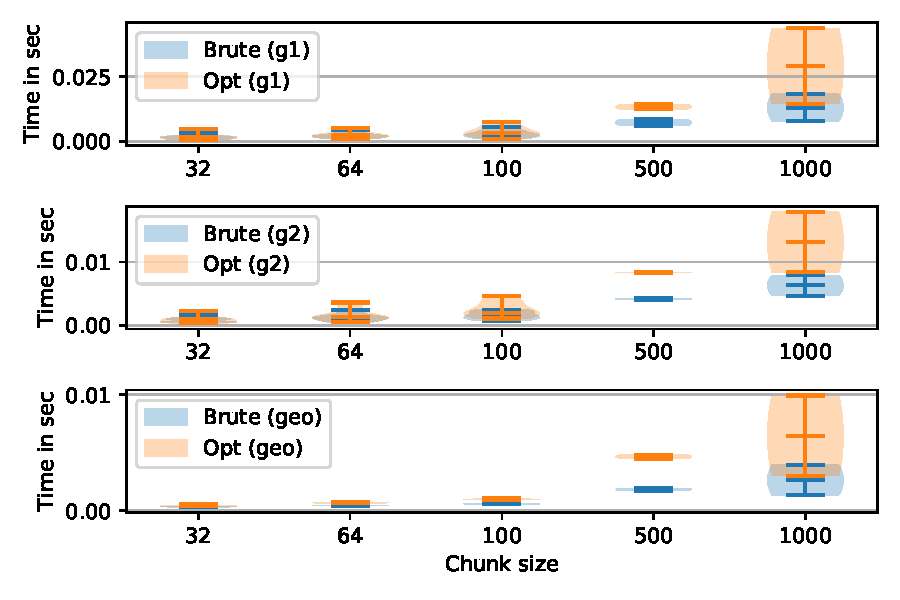
\includegraphics[width=0.5\textwidth]{data/raw/core.pdf}
\caption{Performance of \textit{core} graph querying}
\label{fig:python_core_all}
\end{figure}

\begin{figure}[h]
\centering
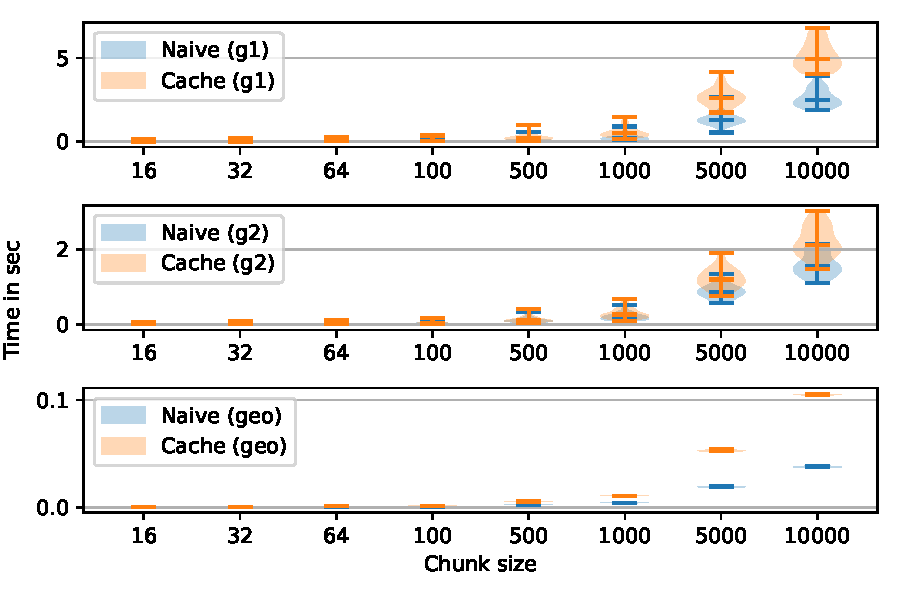
\includegraphics[width=0.5\textwidth]{data/raw/go.pdf}
\caption{Performance of \textit{go} graph querying}
\label{fig:python_go_all}
\end{figure}

\begin{figure}[h]
\centering
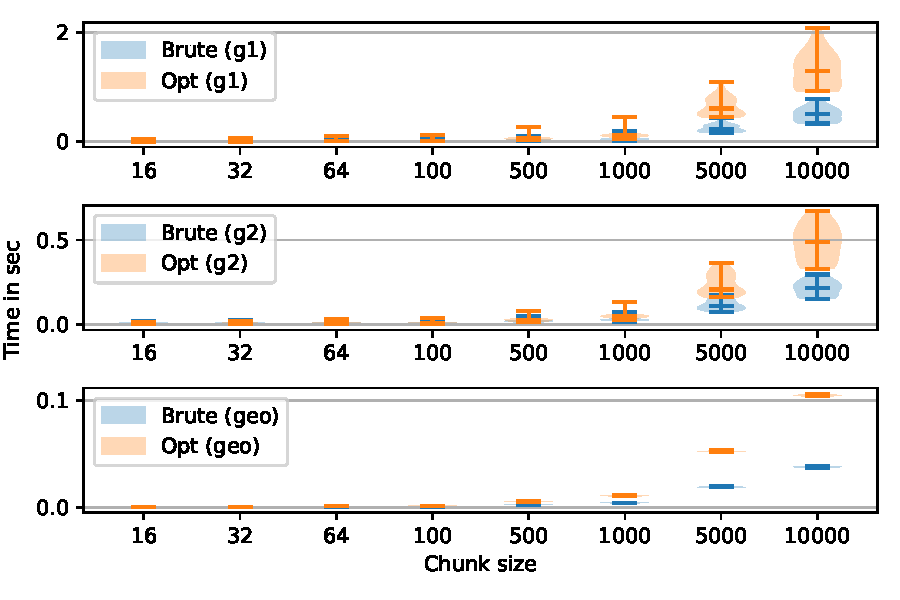
\includegraphics[width=0.5\textwidth]{data/raw/eclass_514en.pdf}
\caption{Performance of \textit{eclass\_514en} graph querying}
\label{fig:python_eclass_all}
\end{figure}

\begin{figure}[h]
\centering
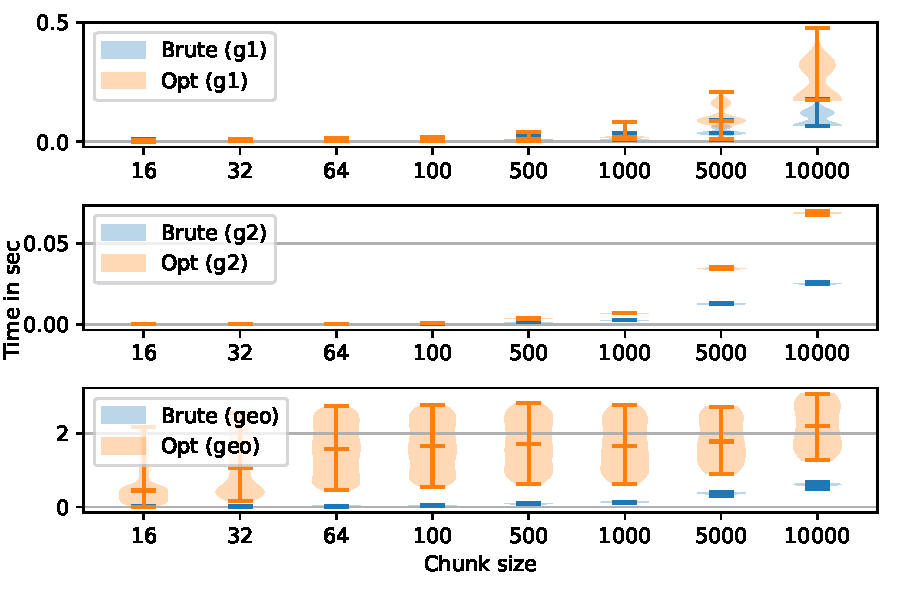
\includegraphics[width=0.5\textwidth]{data/raw/geospecies.pdf}
\caption{Performance of \textit{geospecies} graph querying}
\label{fig:python_geospecies_all}
\end{figure}

\begin{figure}[h]
\centering
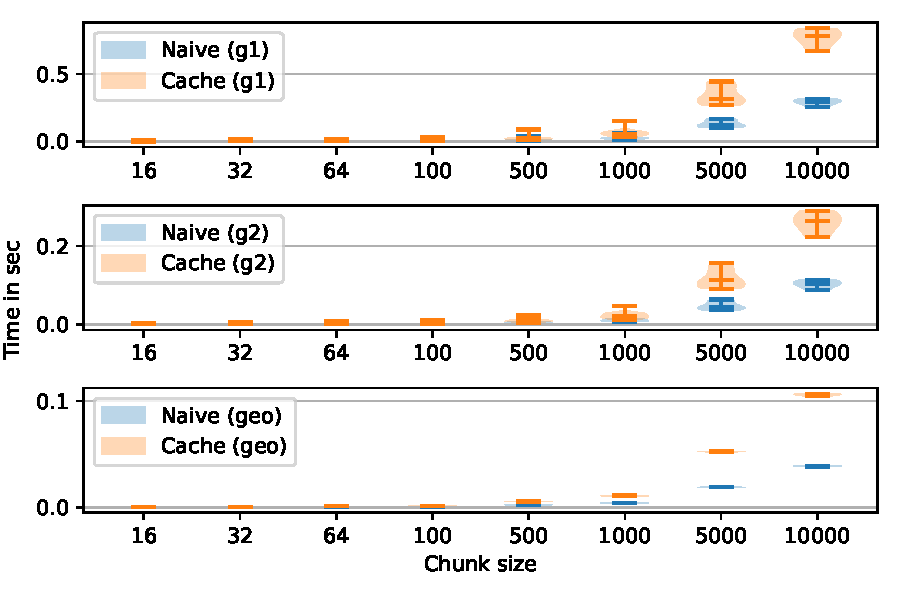
\includegraphics[width=0.5\textwidth]{data/raw/enzyme.pdf}
\caption{Performance of \textit{enzyme} graph querying}
\label{fig:python_enzyme_all}
\end{figure}

\begin{figure}[h]
\centering
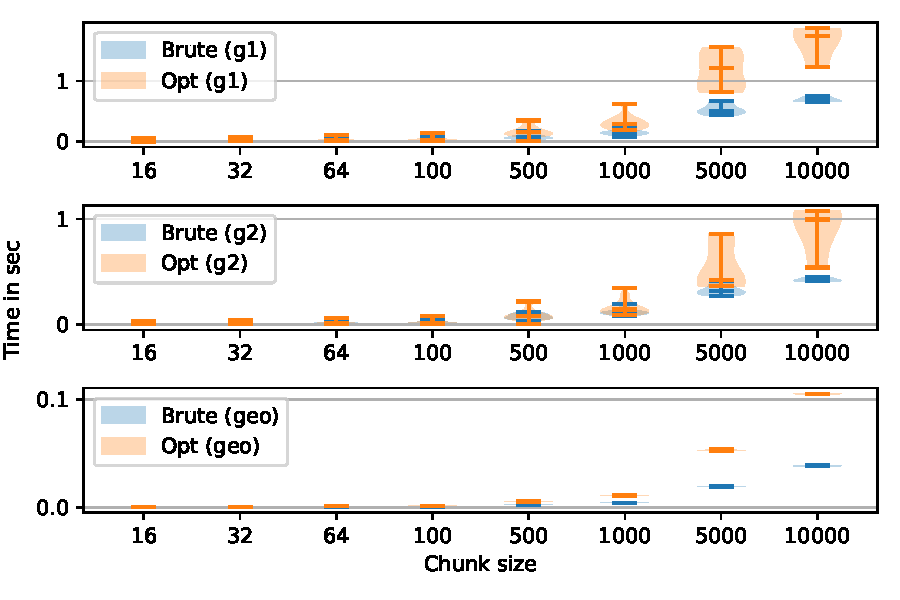
\includegraphics[width=0.5\textwidth]{data/raw/gohierarchy.pdf}
\caption{Performance of \textit{gohierarchy} graph querying}
\label{fig:python_gohierarchy_all}
\end{figure}


\begin{figure}[h]
\centering
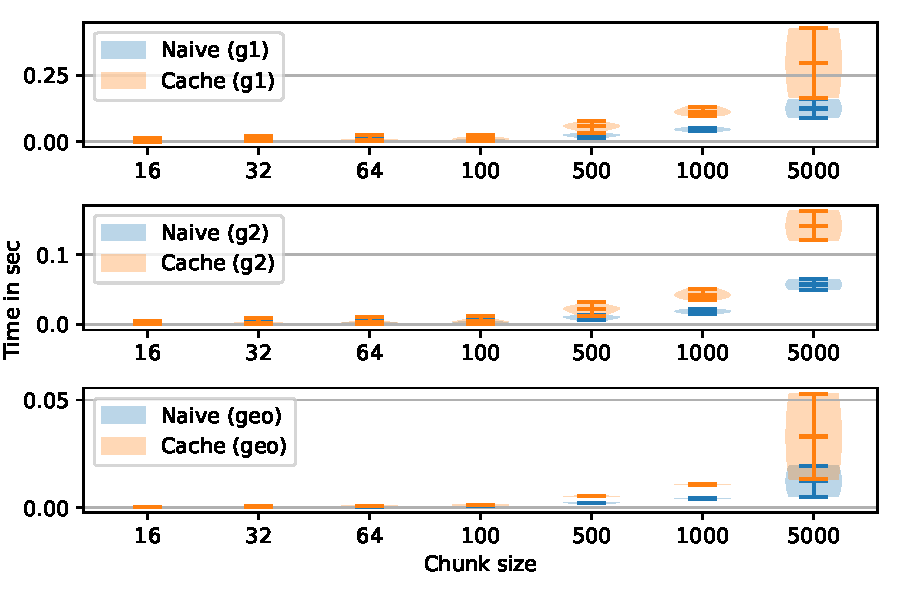
\includegraphics[width=0.5\textwidth]{data/raw/pathways.pdf}
\caption{Performance of \textit{pathways} graph querying}
\label{fig:python_pathways_all}
\end{figure}

\begin{figure}[h]
\centering
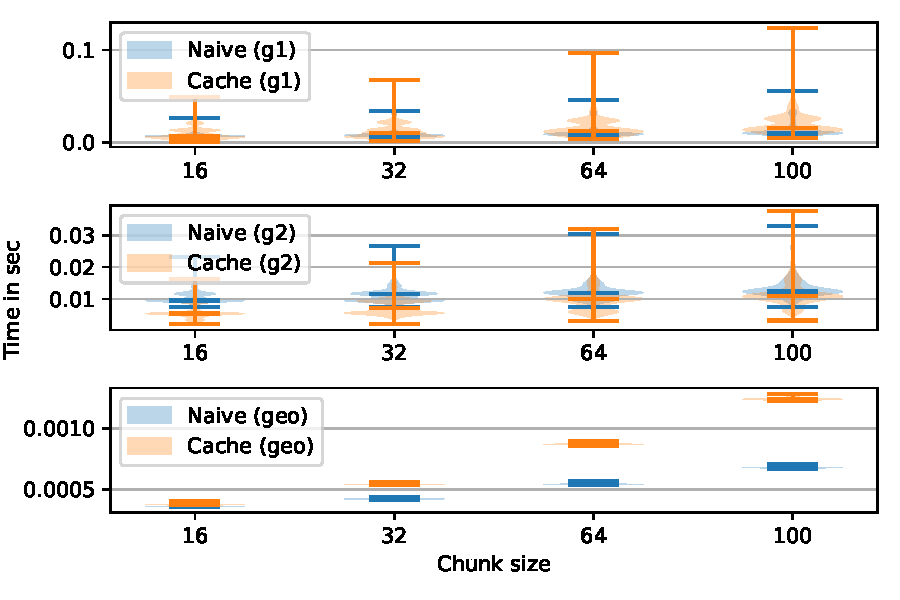
\includegraphics[width=0.5\textwidth]{data/raw/eclass_514en_4.pdf}
\caption{Performance of \textit{eclass\_514en} graph querying with small chunks}
\label{fig:python_eclass_small}
\end{figure}

\begin{figure}[h]
\centering
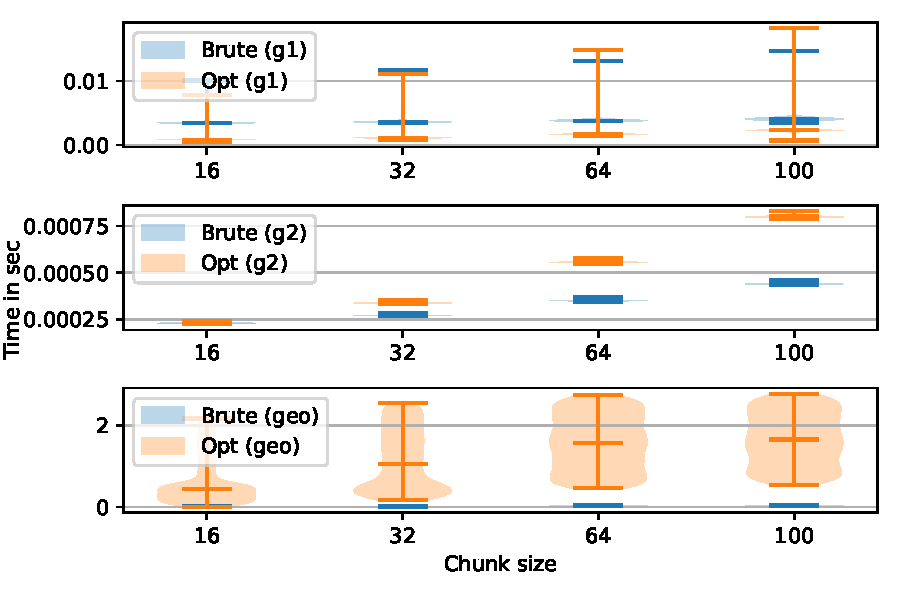
\includegraphics[width=0.5\textwidth]{data/raw/geospecies_4.pdf}
\caption{Performance of \textit{geospecies} graph querying with small chunks}
\label{fig:python_geospecies_small}
\end{figure}

\begin{figure}[h]
\centering
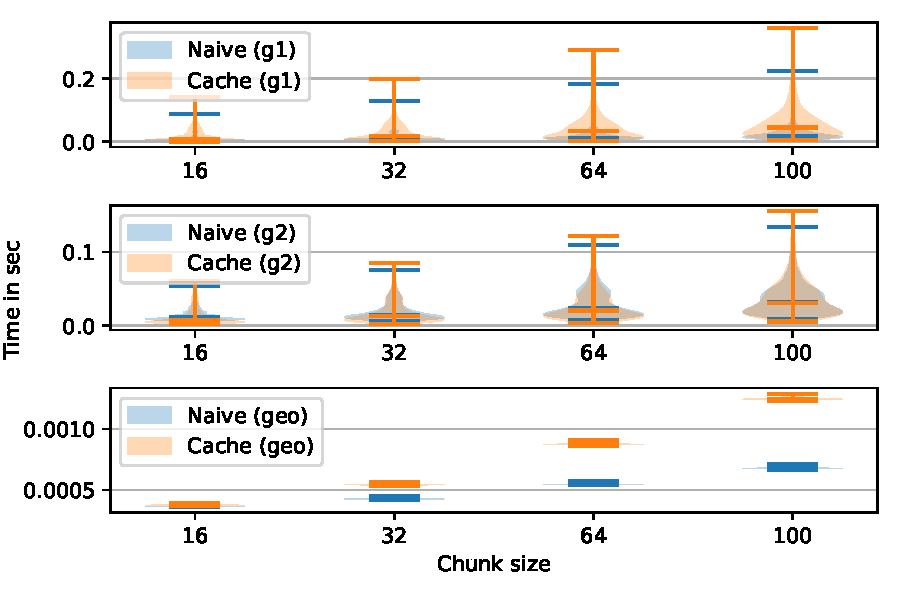
\includegraphics[width=0.5\textwidth]{data/raw/go_4.pdf}
\caption{Performance of \textit{go} graph querying with small chunks}
\label{fig:python_go_small}
\end{figure}


First of all, we can see, that even for cases when graph does not contain edges which are used in query, chunk processing time grows with size of chunk. 
For example, look at the results for \textit{geo} query for all graphs except \textit{geospecies} and \textit{enzyme}.
Thus, preliminary check of existence of edges of interest may be useful in some cases.

Also, we can see, that chunk processing time significantly depends on graph structure. 
For example, for chunks of size $10 000$ and query $g_1$, \textit{go} graph querying requires more than 5 seconds (fig.~\ref{fig:python_go_all}), while \textit{geospecies} graph querying requires less than 0.5 seconds (fig.~\ref{fig:python_geospecies_all}).  

Comparison of two version of algorithm shows that algorithm without caching is significantly faster in almost all cases, even when graph does not contain edges of interest. 
Analysis of results for small chunks (fig.~\ref{fig:python_eclass_small}--\ref{fig:python_go_small}) shows that it is always true. 
For example, for \textit{eclass\_514en} graph and query $g_2$ (fig.~\ref{fig:python_geospecies_small}) median time for algorithm with caching is slightly better than for the na\"{i}ve version.
On the other hand, for \textit{geospecies} graph and $geo$ query (fig.\ref{fig:python_geospecies_small}) algorithm with caching is drastically slower that the na\"{i}ve version.
At the same time, for \textit{go} graph and $g_2$ query median time for both versions are comparable, while time for worst queries is better for the na\"{i}ve version.
Moreover, caching requires additional memory in comparison with na\"{i}ve version of the algorithm.
Thus we can conclude, that query results caching introduces significant overhead and does not lead to significant performance improvements.
Also we can conclude that small chunk processing using the na\"{i}ve version is fast enough: the worst time in our experiments is about 0.2 seconds (fig.~\ref{fig:python_go_small}, query $G_1$). 


As a result, we can conclude that caching is not useful for multiple-source CFPQ for evaluated cases even if one want to process several chunks sequentially, or even process full graph chunk-by-chunk.
Thus, we think that the na\"{i}ve version of the algorithm is better for implementation in real-world graph database. 

